\documentclass{VUMIFPSbakalaurinis}
\usepackage{algorithmicx}
\usepackage{algorithm}
\usepackage{algpseudocode}
\usepackage{amsfonts}
\usepackage{amsmath}
\usepackage{bm}
\usepackage{caption}
\usepackage{color}
\usepackage{float}
\usepackage{graphicx}
\usepackage{listings}
\usepackage{subfig}
\usepackage{wrapfig}
\usepackage{diagbox}
\usepackage{xcolor,colortbl}
\usepackage{fontspec}
\usepackage{enumitem}
\usepackage{multirow}

% Titulinio aprašas
\university{Vilniaus universitetas}
\faculty{Matematikos ir informatikos fakultetas}
\department{Programų sistemų katedra}
\papertype{Bakalauro darbas}
\title{Ryšio mažame lauke naudojimas stacionariame gydyme}
\titleineng{Near field communication in inpatient care}
\status{4 kurso 5 grupės studentas}
\author{Džiugas Baltramėnas}
\supervisor{lekt. Karolis Uosis}
\date{Vilnius – \the\year}

% Nustatymai
%\setmainfont{Time}   % Pakeisti teksto šriftą į Palemonas (turi būti įdiegtas sistemoje)
\bibliography{bibliografija}

\begin{document}
\maketitle

\tableofcontents

\sectionnonum{Įvadas}
Programų sistemų studentai 3 kurse turėjo dalyką, kurio pavadinimas „Programų sistemų kūrimas“, šiame dalyke teko kurti internetinę parduotuvę komandomis. Mūsų komanda buvo pasiskirsčius į 2 grupes, vieni programavo vartotojo sąsają, kiti - vidinį serverį. Mano rolė komandoje buvo vartotojo sąsajos programuotojas ir komandos vadovas. Tai buvo mano pirmoji patirtis kuriant vartotojo sąsają bei dirbant su vartotojo sąsajos technologijomis. Po minėto semestro, supratau, kad savo karjerą noriu tęsti kaip vartotojo sąsajos programuotojas, todėl nusprendžiau savo praktiką atlikti minėtoje pozicijoje. Vartotojo sąsajos programuotojo ieškojo „Tieto“ įmonė, todėl išsiunčiau jiems laišką. „Tieto“ įmonė sutiko mane įdarbinti ir leido atlikti pas juos praktiką. Kadangi įmonė mane įdarbino, už atliekamą praktiką gaudavau atlyginimą, o tai buvo didžiulė motyvacija atlikti savo darbą kaip įmanoma geriau. Susitikus su įmonės praktikos vadovu, buvo aptarta ko įmonė iš manęs tikisi ir kokiame projekte aš dirbsiu. Komandoje, kurios narys aš buvau, dauguma buvo vidutinio (angl. \textit{mid}) ir aukštesniojo (angl. \textit{senior}) lygio programuotojai, todėl tai buvo didžiulė proga mokytis iš šios srities profesionalų. Komandos vadovas buvo paskirtas praktikos mentoriumi. Tam, kad sklandesnis ir greitesnis komunikavimas vyktų tarp mūsų, aš buvau pasodintas šalia jo. Pokalbio su praktikos vadovu metu, aptarėme praktikos tikslą ir uždavinius.

Praktikos tikslas - sukurti interaktyvų kalendorių pamokų, egzaminų ir resursų planavimui bei valdymui.

Išsikelti uždaviniai yra šie:
\begin{itemize}
    \item Atlikti verslo poreikių analizę;
    \item Naudoti ReactJS karkasą, vartotojo sąsajos kūrimui;
    \item Atviro kodo MaterialUI bibliotekos panaudojimas, verslo reikalavimų įgyvendinimui;
    \item Adaptuotų komponentų kūrimas, įgyvendinant sudėtingus verslo poreikius;
    \item Web komponentų testavimas;
    \item Naudotojo sąsajos greitaveikos stebėjimas ir optimizavimas;
\end{itemize}

Visos praktikos metu buvo tobulinamos programavimo, projektavimo, verslo analizės, programų sistemų kūrimo procesų žinios. Projekte, kuriame atlikau praktiką, buvo taikomas vienas iš Agile karkasų - Scrum. Praktikos metu, projektas buvo vykdomas iteracijomis. Vienos iteracijos trukmė - 1 savaitė. Kiekviena iteracija turėjo šiuos etapus:
\begin{itemize}
    \item Iteracijos planavimas;
    \item Užduočių analizavimas ir skaidymas;
    \item Užduočių atlikimas;
    \item Iteracijos užbaigimas;
\end{itemize}
Kiekvienos darbo dienos rytą, buvo atliekamos rytinės diskusijos (angl. \textit{stand-up}), jų metu, kiekvienas komandos narys pasipasakodavo ką atliko praėjusią darbo dieną, su kokiais sunkumais susiduria ir kokias problemas ir uždavinius spręs ateinančią darbo dieną. Jeigu susidurdavau su kažkokiais sunkumais, kurių nepadėdavo išspręsti mentorius, per rytinę diskusiją papasakodavau komandos nariams ir po diskusijos, komandos nariai padėdavo išspręsti problemą. Kiekvieną pirmadienį vykdavo planavimas, kuriame nuspręsdavome kiek per ateinančią savaitę užduočių atliksim ir kiek kiekviena užduotis užtruks laiko. Penktadieniais, darbo pabaigoje, diskutuodavome kaip sekėsi vykdyti planą. Jeigu ne visos suplanuotos užduotys buvo atliktos, diskutavome kokios gali būti priežastys ir kaip to išvengti ateityje. Užduočių valdymui buvo naudojamas „Jira“ įrankis. Šis įrankis leisdavo pamatyti kokios užduotys yra laisvos, kokie jų prioritetai, kurios atliktos užduotys yra testuojamos, o kurios perduotos peržiūrėti klientui.


Kadangi esu tik pradedantysis programuotojas ir didelės darbo patirties neturiu, man buvo sunku įvertinti užduotis, todėl užuot pats pasirinkęs norimą užduotį, man ją parinkdavo komandos vadovas. Praktikos metu atlikau išviso 3 užduotis, 2 iš jų buvo nedidelės, jos skirtos buvo labiau susipažinti su pačiu projektu ir jo struktūra, o trečioji užduotis buvo sudėtingesnė. Paskutinė užduotis buvo išskaidyta į 7 sub-užduotis. Nors komanda dirbo pagal Scrum metodą ir vykdė iteracijas, tačiau mano paskutiniai užduočiai nebuvo taikomos iteracijos, todėl mano užduotis nedidino iteracijos apimties.

\section{„Tieto Lietuva“ įmonė}

\subsection{Įmonės apibūdinimas}
Praktika buvo atlikta įmonės „Tieto“ filiale, kuris yra įsikūręs Lietuvoje. „Tieto“ įmonė įkurta 1968 metais, Suomijoje. Įmonė turi virš 14000 darbuotojų visame pasaulyje, jos filialai yra išsidėstę beveik 20 skirtingose valstybėse, tačiau pagrindiniai filialai ir tikslinė rinka yra Skandinavijos valstybės - Švedija, Suomija ir Norvegija \cite{TIETO}. 2017 metų ataskaitoje minimi šie pagrindiniai faktai, kurie apibūdina įmonę \cite{TIETO}:
\begin{itemize}
    \item Pilnas įmonės pavadinimas yra „Tieto Corporation“;
    \item Įmonės įkūrimo metai yra 1968, jos būstinė bazuojasi Suomijoje, Espe;
    \item Įmonėje dirba daugiau nei 14000 darbuotojų;
    \item Vykdo veiklą 19 šalyse;
    \item Įmonės akcijos yra kotiruojamos Helsinkio NASDAQ akcijų biržoje;
    \item Metinė įmonės apyvarta yra 1,5 milijardų eurų.
\end{itemize}

Verta paminėti tai, jog  „Tieto Corporation“ yra įtrauka į 2018 metų „Thomson Reuters Corporation“ įmonės sudaromą top 100 pasaulio technologijos lyderių sąrašą \cite{List}. Toks įvertinimas rodo tai, jog „Tieto Corporation“ yra pasaulinio mąsto lyderė.

„Tieto Corporation“ užsiimaI tyrimais ir taikomąja veikla (angl. \textit{Research and development, R&D}) šiose pagrindiniuose sektoriuose \cite{TIETO}:
\begin{itemize}
    \item Telekomunikacijų sektoriuje;
    \item Bankininkystės ir draudimo sektoriuje;
    \item Daiktų interneto (angl. \textit{Internet of things, IoT}) sektoriuje;
    \item Sveikatos apsaugos sektoriuje;
    \item Miškų ir energetikos sektoriuje.
\end{itemize}

UAB „Tieto Lietuva“ yra vienas iš 19 „Tieto Corporation“ padalinių. Lietuvoje „Tieto“ savo atstovybę įkūrė 1999 metais. Ši įmonė yra įsikūrusi verslo centre „Park Town“, kurio adresas yra Lvovo g. 105A, Vilnius. Įmonėje dirba apie 120 darbuotojų, UAB „Tieto Lietuva“ generalinis direktorius yra Tomas Vitkus. Įmonės ofise dažniausiai dirba iki 80 darbuotojų, likusieji dirba pas klientus, t.y. dirbama klientų ofisuose. Didžioji dalis vykdomų projektų yra skirti įmonėms, kurios savo veiklą vykdo Lietuvoje. Apie 85\% „Tieto“ klientų yra iš privataus sektoriaus, likusieji - iš viešojo sektoriaus. UAB „Tieto Lietuva“ pagrindinę savo veiklą vykdo šiuose sektoriuose: 

\begin{itemize}
    \item Telekomunikacijų sektoriuje;
    \item Finansų sektoriuje;
    \item Energetikos sektoriuje;
    \item Viešajame sektoriuje;
\end{itemize}

\subsection{Darbo sąlygos}
Verslo centre „Park Town“ yra 9 aukštai, 2 iš šių aukštų yra požeminėje dalyje, kurie yra skirti parkavimo reikmėms. Taip pat viename iš požeminių aukštų yra dušai. „Tieto“ yra įsikūrusi 4 pastato aukšte. Visas 4 aukštas yra naudojamas tik „Tieto“ įmonės. Įmonės ofise nėra kabinetų, todėl darbuotojai gali matyti vieni kitus. Darbuotojai dažnai keičia sėdimas vietas, nes pasikeitus komandai ar projektui neretai yra keičiama ir darbo aplinka. Dažniausiai darbuotojai sėdi kartu su savo komandomis, tačiau įmonėje yra nemažai darbuotojų, kurių komandos yra tarptautinės, todėl dažniausiai darbuotojai sėdi kartu su kitais kolegom, kurių pareigybės yra panašios, t.y. analitikai sėdi vienoje ofiso dalyje, programuotojai ir testuotojai kitoje, administracija dar kitoje, bet yra išimčių. Ofise yra 6 susitiko kambariai (angl. \textit{Meeting room}), kuriuos kiekvienas darbuotojas gali užsirezervuoti. Dirbant atviroje erdvėje, kur nėra kabinetų, pastebėjau, kad sunku susikaupti, dažnai aplink esantys žmonės pradeda itin garsiai kalbėtis, o tai trukdo koncentruotis į atliekamą užduotį. Kadangi ofisas yra nemažas ir nuo vieno galo iki kito užtrunka sąlygiškai nemažai laiko nusigauti, ofise galima rasti paspirtukus, kuriuos darbuotojai gali naudoti keliaujant po ofisą arba keliaujant į miestą pietauti. Taip pat ofise yra virtuvė, kurioje galima šildytis savo atsineštą maistą, išgerti „Tieto“ vaišinama kava, kakava ar chai latte. „Tieto“ įmonė kiekvieną pirmadienį užsako vaisių darbuotojams, vaisiai būna parinkti pagal metų laiką. Dažniausiai vaisių būna tiek, jog jie baigiasi tik trečiadienio pavakarę, todėl darbuotojai gali puse savaitės užkandžiauti vaisiais.

„Tieto“ aprūpina visais darbui reikalingais daiktais: kompiuteriu, jo priedais, monitoriumi, stalu, kėde, kanceliarinėmis priemonėmis ir kt. Jeigu darbuotojas jaučiasi produktyvesnis su keliais monitoriaus, įmonė parūpina, kad darbo vietoje būtų reikiamas kiekis monitorių. Praktikos pradžioje naudojau nemokamą „Visual Studio Code“ integruota kūrimo aplinka (angl. \textit{Integrated Development Environment, IDE}), tačiau paprašius nupirkti „IntelliJ IDEA“, įmonė parūpino šios aplinkos licencija. Šioje įmonėje yra svarbu darbuotojų atlikti darbai, o ne jų išdirbtos valandos, todėl nors darbo sutartyje yra nurodyta jog darbuotoja darbas prasideda 8h, o pasibaigia 17h, tačiau realybėje įmonė nevaržo darbuotojų ir šie gali pradėti ir pabaigti darbą norimu laiku, svarbu, kad paskirti darbai būtų tinkamai atlikti ir mėnesio gale būtų išdirbtas reikiamas valandų skaičius. Kadangi įmonėje visi darbuotojai dirba su nešiojamais kompiuteriais ir įmonei svarbiausia atlikti darbai, „Tieto“ leidžia darbuotojams dirbti iš namų. Man taip pat teko mėginti pasinaudoti šia galimybe, tačiau jaučiausi mažiau produktyvus nei dirbdamas ofise, taip pat buvo sunkiau komunikuoti su komandos nariais, nors visą darbo laiką jie buvo pasiekiami per „Slack“ programėlę. Šie praktikanto aptarti pavyzdžiai parodo, jog įmonė stengiasi sukurti tokias darbo sąlygas, kurios būtų produktyviausios kiekvienam darbuotojui asmeniškai. 

Apibendrinant darbo sąlygas, jos yra puikios, tačiau atviroje erdvėje vykusios diskusijos trukdė susikoncentruoti į atliekamą uždavinį.
\section{Veikla praktikos metu}

\subsection{Vykdomo projekto apibūdinimas}
Praktikos metu studentas dirbo prie projekto, kuris nėra įmonės vidinis projektas, t.y. projektas turi užsakovą. Kadangi praktikantas negali atskleisti užsakovo įmonės pavadinimo, tai draudžia sutartis tarp kliento ir „Tieto“ įmonės, užsakovas bus vadinamas klientu. Klientas vykdo savo veiklą keliose valstybėse, įmonės pagrindinės veiklos yra šios:
\begin{itemize}
    \item Kadetų programa avialinijoms;
    \item Pilotų reitingavimo ir mokymo kursai;
    \item Kitų aviacijos programų mokymai;
\end{itemize}
Kadangi šios įmonės specializacija yra aviacija ir su ja susijusių programų ir kursų vedimas bei veikla vykdoma įvairiose šalyse, natūraliai kyla poreikis susisteminti mokymų valdymą ir koordinavimą. Klientas turi mokymų valdymo sistemą, tačiau jos plėtimo ir palaikymo kaštai yra labai dideli, todėl norint šią sistemą tobulinti, reikia ją perrašyti. Projektas, kuriame studentas dirba, apima tokios sistemos vartotojo sąsajos (angl. \textit{Front-end}) kūrimą. Vidinė sistemos dalis (angl. \textit{Back-end}) su visų galinių punktų (angl. \textit{endpoint}) realizacijomis, yra pateikiama kliento, taip pat klientas suteikia prieigą prie duomenų bazės. Prie šio projekto dirbo 2 komandos, kiekvienoje komandoje buvo po 5-6 programuotojus ir 2 testuotojus, taip pat prie projekto dirbo 1 analitikas ir 1 naudotojų patyrimų dizaineris (angl. \textit{User experience designer}). Dabartinė sistemos vidinė dalis yra parašyta „PHP“ programavimo kalba, „Zend“ karkasu, o vartotojo sąsaja - „Javascript“ programavimo kalba, „Dojo“ karkasu. Komandos, kurioje buvo praktikantas, pagrindinė užduotis buvo sukurti vieną iš sistemos komponentų - kalendorių, ir su juo susijusius funkcionalumus. Kadangi dabartinė sistema turi vartotojo sąsają, kurioje yra realizuotas kalendoriaus funkcionalumas, mūsų tikslas buvo atkartoti esamą kalendorių ir jo funkcionalumus. Taip pat klientas yra išreiškęs norą, kad keletas funkcionalumų būtų kitokie, nei esamoje sistemoje. Skirtingo funkcionalumo reikalavimai buvo dokumentuojami „Jira“ programinėje įrangoje. Pagrindiniai kalendoriaus funkcionalumai yra šie:
\begin{itemize}
    \item Lėktuvų simuliatorių taisymo laiko rezervavimas;
    \item Pamokų organizavimas;
    \item Egzaminų organizavimas;
    \item Studentų įvertinimas;
    \item Visų kalendoriaus objektų laiko koregavimas;
    \item Patalpų rezervavimas;
    \item Darbuotojų darbo laiko rezervavimas;
    \item Priminimų, apie ateinančias įvykius, išsiuntinėjimas.
\end{itemize}

Kiekvieno kalendoriaus objekto kūrimui yra skirtos unikalios formos. Dauguma kalendoriaus objektų turi ne po vieną formą. Visuose formose yra nurodomos pradžios ir pabaigos datos, visi kiti reikalingi duomenys yra unikalūs kiekvienam objektui. Taip pat egzistuoja kalendoriaus objektų, kurie yra susiję su finansais, kaip pavyzdys - pamoka, kiekvienoje pamokoje yra studentų, jie yra apmokestinami. Organizuodami pamoką, vartotojas turi nurodyti pamokos įkainius.

Kalendorius yra interaktyvus, todėl jam yra keliami šie reikalavimai: 
\begin{itemize}
    \item Kalendoriaus objektai turi būti stumdomi (angl. \textit{draggable}) pelytės pagalba;
    \item Kalendoriaus objekto laiko keitimas gali būti atliekamas paspaudus už objekto krašto ir tempiant iki norimo laiko pradžios ir pabaigos;
    \item Stumdymas ir laikų keitimas galimas ne tik vienam objektui, bet ir keliems, t.y. objektus galima pažymėti ir atlikus veiksmus ant vieno objekto, kituose objektuose veiksmai atsikartoja.
    \item Kalendoriaus dienos gali būti keičiamos jas stumdant pelytės pagalba;
    \item Užvedus pelytę ant kalendoriaus objekto, parodoma aktuali informacija.
\end{itemize}

Kalendorius turi filtrus, kurie pagal tam tikrus kriterijus filtruoja kalendoriuje rodomus objektus. Vienas iš filtro reikalavimų - filtro reikšmės turi būti išliekamos (angl. \textit{persistent}), tačiau šios reikšmės nėra saugomos duomenų bazėje. Taip pat mūsų komandai yra paskirta padaryti vadinamus įtaisus (angl. \textit{gadget}). Šie įtaisai rodomi puslapio prietaisų skydelyje (angl. \textit{dashboard}), jie atvaizduoja su kalendoriumi susijusius duomenis. Vieni duomenys yra atvaizduojami grafikais, kiti išrašant į sąrašą. Pagrindiniai įtaisai:
\begin{itemize}
    \item Finansų įtaisas. Šis įtaisas atvaizduoja finansinius duomenis surinktus iš kalendoriau. Duomenys atvaizduojami linijiniu grafiku;
    \item Lėktuvų simuliatorių rezervavimo Įtaisas. Šis įtaisas atvaizduoja kiek kartų ir dėl kokių priežasčių, per pasirinktą laiką, kiekvienas iš simuliatorių buvo rezervuotas. Duomenys atvaizduojami skrituline diagrama;
    \item Egzaminų išlaikymo įtaisas. Šis įtaisas atvaizduoja kiek procentiškai studentų išlaikė pasirinktus egzaminus. Duomenys atvaizduojami stulpeline diagrama;
    \item Artimiausios pamokos. Šis įtaisas atvaizduoja artimiausia pamokas. Duomenys atvaizduojami juos išrašant;
    \item Patalpų užimtumo įtaisas. Šis įtaisas atvaizduoja kiek procentiškai pasirinktos patalpos yra užimtos. Duomenys atvaizduojami stulpeline diagrama.
\end{itemize}

\subsection{Projekto vykdymas}

Projekto įgyvendinimui reikalingos užduotys buvo sugrupuotos ir patalpintos į „Jira“ sistemą. Minėtoje sistemoje talpinami 4 tipų objektai: užduočių grupė, kitaip dar vadinama epiku, užduotis, užduoties sub-užduotis ir klaidos (angl. \textit{bug}). Kiekvienam „Jira“ objektui yra priskiriamas prioritetas, taip nurodoma epikų realizavimo ir klaidų taisymo tvarka. Kodo versijavimui komandos naudojo „Git“ versijų kontrolės sistemą. Kodo saugojimui buvo naudojama „Gitlab“ serveriai. Kiekvienas „Jira“ sistemoje patalpintas objektas buvo identifikuojamas tokiu formatu „MD-XXXX“, kur vietoj „X“ buvo nurodomi skaičiai. Kiekvienai užduočiai/klaidai buvo kuriama atskira atšaka (angl. \textit{branch}), kurios pavadinimas buvo tokiu formatu „md-xxxx-apibūdinimas“ sistemą, kur „md-xxxx“ yra užduoties/klaidos identifikatorius, o „apibūdinimas“ - užduoties/klaidos trumpas, iki 5 žodžių, aprašymas.

Kadangi kliento naudojama sistema buvo labai sunkiai plečiama ir palaikoma, buvo sutarta vartotojo sąsają kurti naudojantis „ReactJS“ biblioteka ir „Typescript“ kalba, šios technologijos padėjo pasiekti lengvą sistemos palaikomumą ir plečiamumą. Kadangi „ReactJS“ bibliotekos globalių būsenų valdymas nėra trivialus, pasirinkta naudoti „Redux“ globalių būsenų valdymo biblioteką. Vienas iš pagrindinių sistemos komponentų - formos, kadangi buvo pasirinkta naudoti „Redux“ biblioteką, formų valdymui buvo pasirinkta naudoti „Redux Form“ biblioteką, kuri visas formų būsenas, jų reikšmes, laiko globalioje būsenoje. Tinkamo puslapio vaizdavimui (angl. \textit{routing}), buvo naudojama „React-router“ biblioteka. Komunikavimui, tarp vartotojo sąsajos ir serverio, buvo pasirinkta naudoti „Axios“ biblioteką. Klientui, vartotojo sąsajoje yra svarbiausias funkcionalumas, todėl nereikalavo unikalių dizaino sprendimų. Vartotojo sąsajos grafinių elementų kūrimui buvo naudojama „MaterialUI“ biblioteka. Komponentų vienetų testų rašymui ir leidimui buvo naudojamos „Jest“ ir „Enzyme“ bibliotekos, o automatiniams testams buvo naudojamas „Selenium“ karkasas. Kadangi klientas vykdo savo veiklą įvairiose pasaulio valstybėse, kuriamą sistemą naudosis ne tik Lietuvoje. Tam, kad darbuotojai, kurie nemoka lietuvių kalbos, galėtų naudotis kuriama sistema, buvo pasirinkta naudoti „i18n“ biblioteką, kuri pasirūpintų tekstų vertinimu. Komunikacijos protokolas, tarp vidinio serverio ir vartotojo sąsajos, buvo skirtingas skirtinguose puslapio vietose. Vienur naudojamas „REST“, o kitur, tame tarpe ir kalendoriuje, „JSON-RPC 2.0“ protokolas.

Studentas praktikos metu prisidėjo prie kalendoriaus ir įtaisų kūrimo. Pagrindinės užduotys, kurias studentas atliko kurdamas kalendorių yra šios: 
\begin{itemize}
    \item Priminimų išsiuntimas;
    \item Darbuotojų laiko rezervavimo formos kūrimas.
\end{itemize}

Pirmiausiai praktikantas atliko priminimų išsiuntimo užduotį. Kuriamas kalendorius yra atvaizduojamas lentelėje. Stulpeliai reprezentuoja laiką, eilutės - dieną. Kalendoriaus vienoje eilutėje atvaizduojamos visos 24 valandos, tačiau vartotojas gali pasirinkti ar kalendorius laiką atvaizduoti kas 15 minučių, ar kas 1 valandą. Kiekviena eilutė turi laiško ikoną, paspaudus šią ikoną užfiksuojama kurioje dienoje ikona buvo paspausta. Kadangi visi kalendoriaus duomenys buvo laikomi globalioje būsenoje, praktikantui reikėjo pagal užfiksuotą dieną išfiltruoti ir atrinkti tik tuos duomenis, kurie patenka į tos dienos rėžius. Jeigu kalendoriaus objekto pradžia ir pabaiga yra skirtingose dienose, bet vienas iš jų patenka į užfiksuotą dieną, objektas įtraukiamas į objektų sąrašą, kuriems bus išsiųstas priminimas. Turint reikiamus kalendoriaus objektus, praktikantas siunčia visų kalendorių identifikacijos numerius vidiniam serveriui su metodo parametro reikšme „sendNotification“.

Atliekant antrą užduotį, praktikantui reikėjo suprogramuoti vieną iš kalendoriaus formų. Formai yra reikalingi 4 skirtingi formos komponentai:
\begin{itemize}
    \item Datos parinkimo komponentas;
    \item Paprastas teksto įvedimo komponentas;
    \item Komponentas su pasirinkimo variantais (angl. \textit{select component});
    \item Žymimojo langelio (angl. \textit{checkbox}) komponentas.
\end{itemize} 
Tam, kad naudoti formos komponentus kartu su „Redux form“ biblioteka, kiekvieną komponentą reikėjo pritaikyti prie šios bibliotekos. Kuriant paskirtą formą, visi reikalingi komponentai jau buvo sukurti, todėl studentui užteko juos paimti ir panaudoti formoje. Sukūrus formą, visi duomenys buvo suformuojami taip, kad būtų tinkami vidiniam serveriui ir duomenų bazei. Turint reikiamo formato duomenis, jie yra siunčiami vidiniam serveriui, o vartotojui yra pranešama, kad rezervacija atlikta.

Praktikos eigoje studentui buvo skirta dar viena užduotis - sukurti prietaisų skydelio infrastruktūrą. Ši užduotis buvo pati plačiausia, reikalaujanti daugiausiai studento pastangų ir laiko. Kadangi pagrindinė problema, kurią sprendėme kurdami naują sistemą, yra sistemos plečiamumas, įtaisų infrastruktūrą reikėjo sukurti tokią, kurioje būtų lengva pridėti ir kurti naujus įtaisus. Studentas, analizuodamas dabartinę įtaisų situaciją, turėjo analizuoti senosios sistemos įtaisų kodą, nes pilnas įtaisų funkcionalumas nebuvo akivaizdus vien tik analizuojant senosios sistemos vartotojo sąsają. Nagrinėjant senąjį kodą, buvo išsiaiškinti funkcionalumai, kurie yra bendri visiems įtaisams:
\begin{itemize}
    \item Kiekvienas įtaisas atnaujina rodomus duomenis kartą per nurodytą laiką. Atsinaujinimo periodas yra įkoduotas (angl. \textit{hard coded}) į sistemą. Kiekvienas įtaisas turėjo įkoduotą periodą, dauguma įtaisų turėjo įkoduotą 60 minučių periodą, keletas - 20 minučių, taip pat buvo 1 įtaisas, kurio atsinaujinimo periodas yra 1 min.
    \item Įtaisai užima visą prietaisų skydelio plotą arba puse. Kiekvienas įtaisas turi įkoduotą užimamą plotą. Visą plotą užimantys įtaisai turi ploto parametrą su „full“ reikšme, o puse ploto užimantys įtaisai turi parametrą su „half“ string tipo reikšme.
    \item Įtaisų išdėstymo tvarka yra nurodoma vidinio sistemos serverio. Kiekvienas naujai pridedamas įtaisas dedamas į įtaisų eilės galą. Visi įtaisai gali būti sukeisti vietomis arba įtaisai gali būti įterpiami tarp dviejų kitų įtaisų. Eilės tvarkos keitimas yra atliekamas „drag and drop“ principu.
    \item Dauguma įtaisų turi filtrus, kuriuos pakeitus, vaizduojami duomenys filtruojami pagal pasirinktus filtrus. Dauguma įtaisų turi lėktuvo simuliatoriaus ir periodo filtrus.
    \item Visų įtaisų konfigūracija yra valdoma sistemos naudotojo. Pakeitus įtaiso konfigūraciją, naudotojas privalo paspausti mygtuką „Išsaugoti“. 
\end{itemize}

Įdomu yra tai, kad kiekvieno filtro ir konfigūracijos reikšmės buvo saugomos duomenų bazėje, o kiekvieną kartą pakeitus įtaiso filtrą ar konfigūraciją, reikėjo siųsti vidiniam serveriui vieną užklausa, kurioje buvo nurodomi visi įtaisai su visomis filtrų ir konfigūracijų reikšmėmis. Išimant įtaisą iš prietaisų skydelio, reikėjo siųsti tą pačią užklausą, tačiau iš įtaisų sąrašo išimant norimą įtaisą. Apskritai, visas prietaisų skydelio valdymas buvo atliekamas viena užklausa, kurioje tik duomenys skyrėsi.

Analizuojant prietaisų skydelio funkcionalumą, studentui nebuvo aišku pagal kokius kriterijus prietaisų skydelis vaizduoja įtaisus. Buvo pastebėta, kad skirtingi vartotojai mato skirtingą įtaisų kiekį, tačiau nebuvo aišku kodėl kiekis skiriasi. Tam, kad išsiaiškint minėtus dalykus, praktikos vadovo buvo paprašyta suorganizuoti praktikanto susitikimą su klientu. Keliu dienų bėgyje buvo suorganizuotas internetinis pokalbis. Klientas praktikantui paaiškino, jog kiekvienas įtaisas turi leidimus (angl. \textit{permissions}). Jeigu vartotojas neturi reikalingų leidimų matyti įtaisus, jis jų nemato. Visų šių leidimų valdymas yra atliekamas vidinėje serverio dalyje, todėl papildomų sunkumų, kuriant prietaisų skydelio infrastruktūrą, neiškilo. Studentas, spręsdamas gautą užduotį, braižėsi preliminarias architektūras, tačiau jos buvo braižomas padrikai ir nesilaikant „UML“ taisyklių. Brėžiniai buvo rodomi ir tikslinami su komandos vadovu. Komandos vadovas padėjo išspręsti kilusius sunkumas, tačiau patarė pabandyti suprogramuoti ir validuoti nubraižytą architektūrą. Praktikantas suprogramavęs architektūra, sukūrė „Merge request“ tam, kad kiti komandos nariai galėtų pažiūrėti ir įvertinti sukurtą infrastruktūrą. Pagal parašytas pastabas, praktikantas patobulino siūlomą architektūrą ir užduoties atšaką sujungė su pagrindine kodo atšaka. Suprogramuotos prietaisų skydelio architektūros diagrama yra pavaizduota žemiau (žiūrėti 1 pav.).


\begin{figure}[H]
    \centering
    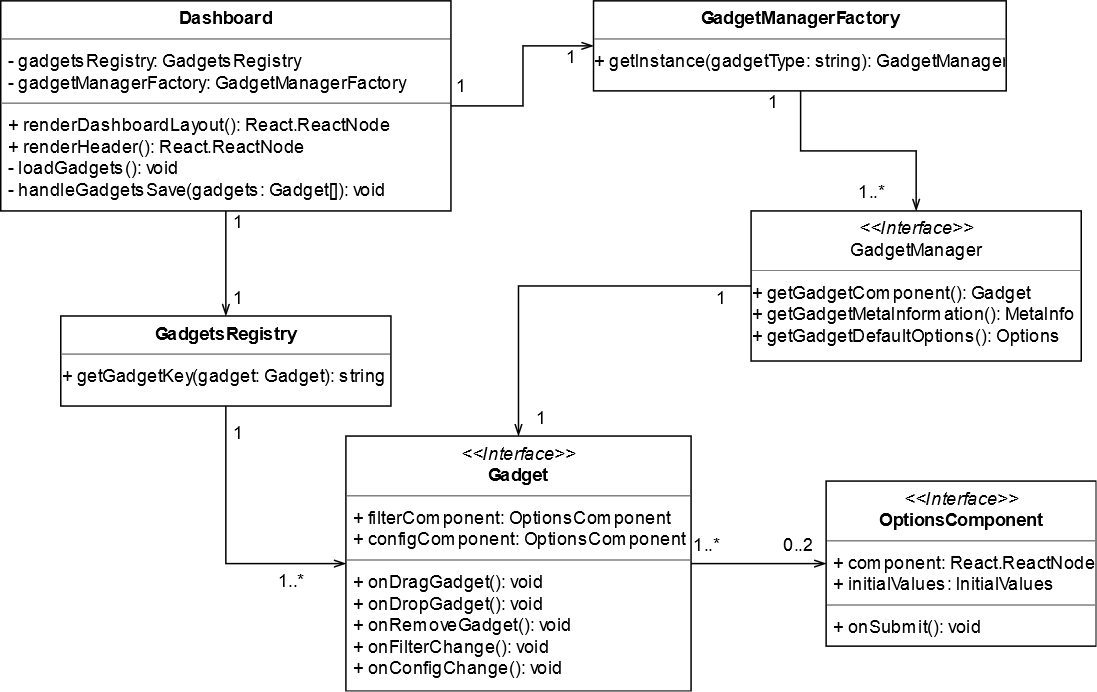
\includegraphics[scale=0.45]{images/gadgets}
    \caption{Prietaisų skydelio ir įtaisų infrastruktūros architektūra} 
\end{figure}

\begin{itemize}
    \item Klasė „\textbf{Dashboard}“. Ši klasė atsakinga už visų įtaisų atvaizdavimą (angl. \textit{render}). Tam, kad sužinotų kokius įtaisus reikia atvaizduoti, pirmiausiai ši klasė kreipiasi į vidinį serverį su „JSON-RPC 2.0“ protokolo užklausa, kurios metodo parametro reikšmė yra „getTemplate“, serveris grąžina šablono (angl. \textit{template}) identifikacijos numerį. Kiekvienas vartotojas turi savo unikalų šablono identifikacijos numerį. Gavus šablono numerį, ši klasė kreipiasi dar kartą į vidinį serverį, šioje užklausoje metodo parametro reikšmė yra „getGadgets“, taip pat nurodomas šablono numeris. Įvykdžius šias dvi užklausas, klasė turi informaciją apie įtaisus, kuriuos reikia atvaizduoti. Yra atvejų, kuomet gauti įtaisai neturi identifikacijos numerio, tokiu atveju jiems yra taikomos numatytos (angl. \textit{default}) konfigūracijos, tačiau architektūros implementacijoje yra reikalaujama, kad kiekvienas įtaisas turėtų identifikacijos numerį. Kiekvienam įtaisui unikalus numeris yra paskiriamas klasės „GadgetsRegistry“. Galiausiai, klasė kreipiasi į „GadgetManagerFactory“ klasę, kuri grąžina norimo įtaiso komponentą. Turint visų įtaisų komponentus, „Dashboard“ klasė juos atvaizduoja.
    \item Klasė „\textbf{GadgetsRegistry}“. Ši klasė yra atsakinga, kad visi atvaizduojami įtaisai turėtų unikalius numerius, kurie naudojami kaip komponentų raktai (angl. \textit{key}). Jeigu nurodomas įtaisas neturi identifikacijos numerio, ši klasė pati sugeneruoja numerį ir priskiria nurodytam įtaisui. Jeigu įtaisas turi identifikacijos numerį, ši klasė grąžina jį.
    \item Klasė „\textbf{GadgetManagerFactory}“. Ši klasė yra tarpinė tarp klasės „Dashboard“ ir „GadgetManager“. Ši klasė žino apie visus implementuotus įtaisus. Kiekvienas įtaisas turi savo tipą. Nurodant įtaiso tipą, ši klasė grąžina įtaiso valdiklį (angl. \textit{manager}). 
    \item Interfeisas „\textbf{GadgetManager}“. Kiekvienam įtaisui yra paskirtas valdiklis. Valdikliai yra atsakingi už įtaiso komponento grąžinimą, įtaiso meta informacijos grąžinimą ir įtaiso numatytų konfigūracijų grąžinimą. Visi įtaisų valdikliai implementuoja šį „GadgetManager“ interfeisą.
    \item Interfeisas „\textbf{OptionsComponent}“. Dauguma įtaisų turi filtrus ir konfigūracijas. Tiek filtrai, tiek konfigūracijos yra sudaryti iš formų ir gali turėti pradines reikšmes. Vienintelis skirtumas tarp filtrų ir konfigūracijų - įtaisas iškart reaguoja į filtro pakeitimą, o pakeitus konfigūraciją, reikia paspausti mygtuką „Išsaugoti“. Visi filtrų ir konfigūracijų komponentai įgyvendina šį interfeisą.
    \item Interfeisas „\textbf{Gadget}“. Visų įtaisų eilės tvarka yra koreguojama „Drag and drop“ principu, todėl visi įtaisai turi interfeiso „drag“ ir „drop“ metodus. Taip pat visus įtaisus galima pašalinti iš įtaisų sąrašo ir dauguma įtaisų turi filtrus ir konfigūracijas. Šį interfeisą įgyvendina visų įtaisų komponentai.
\end{itemize}

Tam, kad būtų aišku, kaip įtaisai turi būti implementuoti, studentui buvo duota užduotis sukurti 3 įtaisus. Vienas iš įtaisų atvaizduoja savo duomenis lentelės formatu, kitas - skrituline diagrama, o trečias linijine diagrama. Atvaizduoti duomenis lentelėje buvo paprasčiausia. Duomenų atvaizdavimui buvo naudojamas „MaterialUI“ lentelės komponentas. Praktikantui sudėtingiau sekėsi atvaizduoti duomenis diagramose. Diagramų braižymui buvo pasirinkta naudoti „Recharts“ biblioteką. Tam, kad pavaizduoti diagramas, pakako perduoti duomenis vienam iš bibliotekos komponentų, tačiau sudėtingiausia buvo suformuoti legendą ir atvaizduoti duomenis ant diagramos elementų. Buvo norima, kad ant diagramos kraštinės būtų nurodomi duomenys. Linijinės diagramos atveju, tai padaryti nebuvo sudėtinga, tačiau programuojant skritulinę diagramą, kilo sunkumų. Kadangi skritulinė diagrama sudaryta iš apskritimo, reikėjo prisiminti sinusų ir kosinusų teorijas. Linijinėje diagramoje sudėtingiausia buvo suformuoti x ir y ašis, kadangi šias ašis reikėjo atvaizduoti kitaip nei biblioteka formatavo. Suprogramavus įtaisus, praktikantas sukūrė šių įtaisų komponentų vienetų testus.

\section{Rezultatai, išvados, pasiūlymai ir pastabos}

\subsection{Rezultatai}
Nors praktikos tikslas buvo - sukurti interaktyvų kalendorių pamokų, egzaminų ir resursų planavimui bei valdymui, tačiau praktikos metu tik nedidelę dalį savo laiko praktikantas skyrė kurdamas kalendorių, didžiausią laiko dalį praktikantas skyrė netiesiogiai su kalendoriu susijusių funkcionalumų kūrimui, todėl galima teigti, kad išsikeltas tikslas yra pasiektas. Buvo išnagrinėta kliento pasenusi (angl. \textit{legacy}) sistema tam, kad suprasti paslėptą funkcionalumą, tai leido tobulinti praktikanto gebėjimą skaityti svetimą kodą. Praktikos metu, buvo suprojektuota ir suprogramuota prietaisų skydelių architektūra, kuri pradėta naudoti realioje sistemoje.

\subsection{Išvados}
Praktikos metu, studentas įgijo daug programavimo ir projektavimo patirties. Praktikantas, analizuodamas keliamus reikalavimus ir bendraudamas su klientu, pagerino savo analitinius sugebėjimus ir formalaus bendravimo įgūdžius. Studentas įgijo ir pagilino savo žinias šiuose aspektuose:

\begin{itemize}
    \item Kodo versijavime;
    \item Architektūrų projektavime;
    \item Komandiniame darbe;
    \item „ReactJS“ ir „Typescript“ programavime;
    \item Vartotojo sąsajos komponentų vienetų testų rašyme;
    \item Svetimo kodo skaityme;
    \item Grafikų programavime su „Recharts“ biblioteka;
    \item Formaliame bendravime;
\end{itemize}

\subsection{Pasiūlymai ir pastabos}
„Tieto“ įmonės suteikta praktika buvo puiki, jokių priekaištų neturiu. Labai džiaugiuosi, kad komanda davė daug laisvės ir nevaržė atliekant praktiką. Praktikos metu susidūriau su daug naujų technologijų, todėl praktikos pradžioje reikėjo keleto savaičių įsivažiuoti, labai džiaugiuosi, kad turėjau puikų mentorių, kuris visada pagelbėdavo. Mano manymu, universitete dėstomos medžiagos pakanka tam, kad studentai greitai prisitaikytų darbo vietoje, nes juk universitetas moko mokytis, o tai ir yra svarbiausia dirbant prie realių projektų.
 
\printbibliography[heading=bibintoc]  % Šaltinių sąraše nurodoma panaudota
% literatūra, kitokie šaltiniai. Abėcėlės tvarka išdėstomi darbe panaudotų
% (cituotų, perfrazuotų ar bent paminėtų) mokslo leidinių, kitokių publikacijų
% bibliografiniai aprašai.  Šaltinių sąrašas spausdinamas iš naujo puslapio.
% Aprašai pateikiami netransliteruoti. Šaltinių sąraše negali būti tokių
% šaltinių, kurie nebuvo paminėti tekste.


\end{document}
